
\documentclass{article}
\usepackage{amsmath, amssymb, graphicx, subcaption, listings,xcolor}  % For \mathbb command

\definecolor{codegreen}{rgb}{0,0.6,0}
\definecolor{codegray}{rgb}{0.5,0.5,0.5}
\definecolor{codepurple}{rgb}{0.58,0,0.82}
\definecolor{backcolour}{rgb}{0.95,0.95,0.92}

\lstdefinestyle{mystyle}{
    backgroundcolor=\color{backcolour},   
    commentstyle=\color{codegreen},
    keywordstyle=\color{magenta},
    numberstyle=\tiny\color{codegray},
    stringstyle=\color{codepurple},
    basicstyle=\ttfamily\footnotesize,
    breakatwhitespace=false,         
    breaklines=true,                 
    captionpos=b,                    
    keepspaces=true,                 
    numbers=left,                    
    numbersep=5pt,                  
    showspaces=false,                
    showstringspaces=false,
    showtabs=false,                  
    tabsize=2
}

\lstset{style=mystyle}


    \title{Practicas MC}
    \date{\today}
    \author{Juan Luis Torres Ramos}

    \begin{document}
        
        % 
        % Portada
        % \pagenumbering{gobble}
        % \maketitle
        % \newpage
        % \pagenumbering{arabic}

        \begin{titlepage}
            \centering
            {
\includegraphics[width=1\textwidth]{./Imagenes/logo_universidad_de_granada.png}\par}
            \vspace{1cm}
            {\scshape\Large Escuela Tecnica Superior de Ingenieria Informatica y Telecomunicaciones \par}
            \vspace{2.5cm}
            {\scshape\Huge Practicas Modelos de Computación \par}
            \vspace{1cm}
            {\itshape\Large  Grupo B3 \par} 
            \vfill
            {\Large Juan Luis Torres Ramos \par}
            \vspace{0.5cm}
            {\large 24 Octubre 2023 \par}
            \end{titlepage}


        % introducción
        \section*{Practica 1}
        Encuentra una gramática libre del contexto para generar cada uno de los siguientes lenguajes:

        \begin{enumerate}
            \item $L = \{a^i b^j \, | \, i, j \in \mathbb{N}, \, i \leq j\}$.
            \item $L = \{a^i b^j a^j b^i \, | \, i, j \in \mathbb{N}\}$.
            \item $L = \{a^i b^i a^j b^j \, | \, i, j \in \mathbb{N}\}$.
            \item $L = \{a_i b_i \,|\, i \in \mathbb{N}\} \cup \{b_i a_i \,|\, i \in \mathbb{N\}}$.
            \item $L = \{uu^{-1} \mid u \in \{a, b\}^*\}$.
            \item $L = \{a^i b^j c^{i+j} \, | \, i, j \in \mathbb{N}\}$.    
        \end{enumerate}

        \begin{flushleft}
            donde $\mathbb{N}$ es el conjunto de los numeros naturales incluyendo el 0
        \end{flushleft}

        \vspace{\baselineskip} % paso linea

        % Pasos que voy a seguir para resolver el ejercicio
        \begin{flushleft}
            
            \subsubsection*{Pasos para resolver el ejercicio:}
                        
            \begin{enumerate}
                \item Determinar los símbolos terminales y no terminales.
                \item Determinar el símbolo inicial.
                \item Analizar el lenguaje para determinar qué se pide.
                \item Determinar las reglas de producción.
                \item Comprobar con JFLAP  
            \end{enumerate}
        \end{flushleft}


        \newpage

        % 
        % APARTADO 1

        \subsection*{A. $L = \{a^i b^j \, | \, i, j \in \mathbb{N}, \, i \leq j\}$.}

        \begin{flushleft}
            \begin{enumerate}
                \item Los símbolos terminales serán $\{a,b\}$ y los simbolos no terminales serán $S$ y $B$.
                \item El símbolo inicial será $S$.
                \item Analizar el lenguaje para determinar qué se pide. En este caso, se pide que la cadena tenga un número de $a$ menor o igual que el número de $b$. Por ejemplo, $aabbb$ y $aabb$ pertenecen al lenguaje, pero $aab$ no.
                \item Determino las reglas de producción:
                \begin{itemize}
                    \item $S \rightarrow \epsilon$ (genero la cadena vacía).
                    \item $S \rightarrow aSb$.
                    \item $S \rightarrow Sb$.
                \end{itemize}

                \item compruebo con JFLAP que la gramática es correcta.
                
                \vspace{\baselineskip} % paso linea

                % Imagenes en matriz
                \begin{figure}[h] 
                    \centering
                    \begin{subfigure}[b]{0.45\textwidth}
                        \centering
                        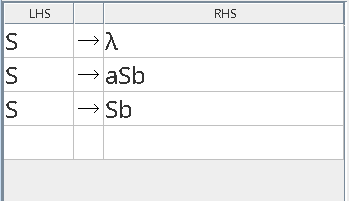
\includegraphics[width=\textwidth]{./Imagenes/produccion1.png}
                        \caption{la producción}
                        \label{fig:label1}
                    \end{subfigure}
                    \hfill
                    \begin{subfigure}[b]{0.45\textwidth}
                        \centering
                        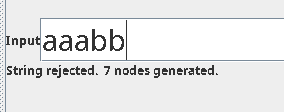
\includegraphics[width=\textwidth]{./Imagenes/grafoaaabb.png}
                        \caption{la cadena $aaabb$}
                        \label{fig:label2}
                    \end{subfigure}
                    \vspace{0.5cm} 
                    \\
                    \begin{subfigure}[b]{0.45\textwidth}
                        \centering
                        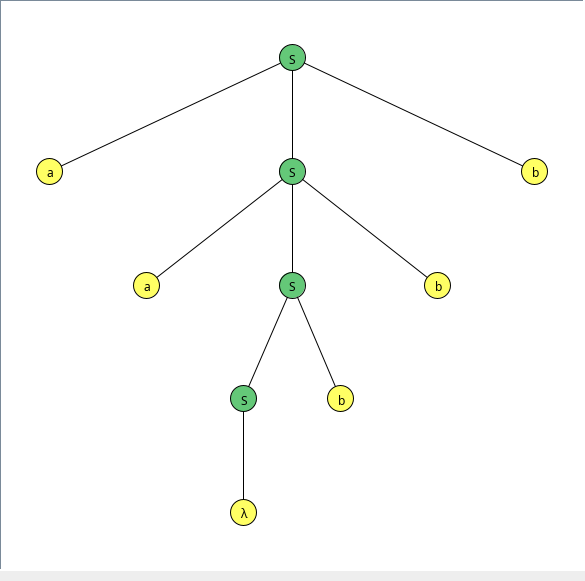
\includegraphics[width=\textwidth]{./Imagenes/grafoaabbb.png}
                        \caption{la cadena $aabbb$}
                        \label{fig:label3}
                    \end{subfigure}
                    \hfill
                    \begin{subfigure}[b]{0.45\textwidth}
                        \centering
                        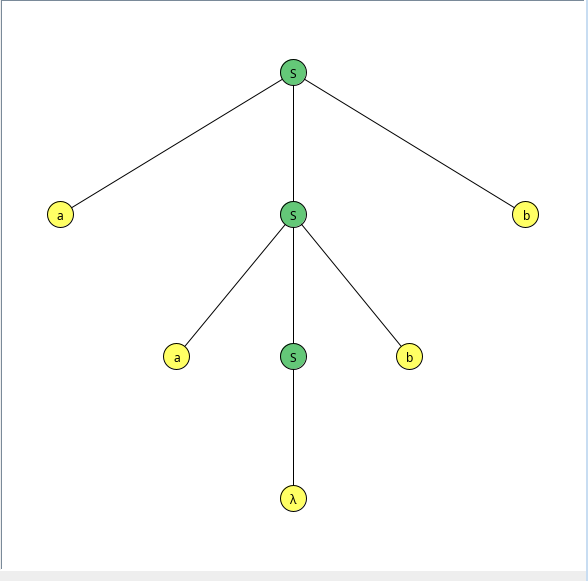
\includegraphics[width=\textwidth]{./Imagenes/grafoaabb.png}
                        \caption{la cadena $aabb$}
                        \label{fig:label4}
                    \end{subfigure}
                    \label{fig:matrix1}
                \end{figure}

                

                 

            \end{enumerate}
        \end{flushleft}

        % 
        % Apartado 2

        \newpage % paso pagina
        \subsection*{B. $L = \{a^i b^j a^j b^i \, | \, i, j \in \mathbb{N}\}$.}
        \begin{flushleft}
            \begin{enumerate}

                \item Los símbolos terminales serán $\{a,b\}$ y los simbolos no terminales serán $S$ y $B$.

                \item El símbolo inicial será $S$.
            
                \item El lenguaje nos pide generar una cadena de 4 caracteres donde primero se generen $a^i b^j$ y luego $a^j b^i$, es decir en los extremos un numero caracteres $i$ y en los caracteres del centro un numero de caracteres $j$. 
                Por ejemplo, $aababb$ y $ab$ pertenecen al lenguaje, pero $aabbab$ no.

                \item Determino las reglas de producción:
                \begin{itemize}
                    \item $S \rightarrow aSb$ (genero mismo numero de caracteres en los extremos).
                    \item $S \rightarrow B$.
                    \item $B \rightarrow bBa$ (genero mismo numero de caracteres en el centro).
                    \item $B \rightarrow \epsilon$ (genero la cadena vacía).
                \end{itemize}

                \item compruebo con JFLAP que la gramática es correcta.

                % Imagenes en matriz
                \begin{figure}[h] 
                    \centering
                    \begin{subfigure}[b]{0.45\textwidth}
                        \centering
                        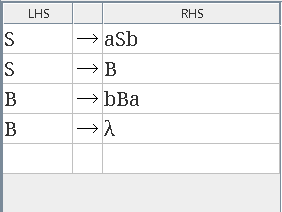
\includegraphics[width=\textwidth]{./Imagenes/produccion2.png}
                        \caption{la producción}
                        \label{fig:label5}
                    \end{subfigure}
                    \hfill
                    \begin{subfigure}[b]{0.45\textwidth}
                        \centering
                        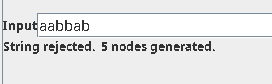
\includegraphics[width=\textwidth]{./Imagenes/grafo3.png}
                        \caption{la cadena $aabbab$}
                        \label{fig:label6}
                    \end{subfigure}
                    \vspace{0.5cm} 
                    \\
                    \begin{subfigure}[b]{0.45\textwidth}
                        \centering
                        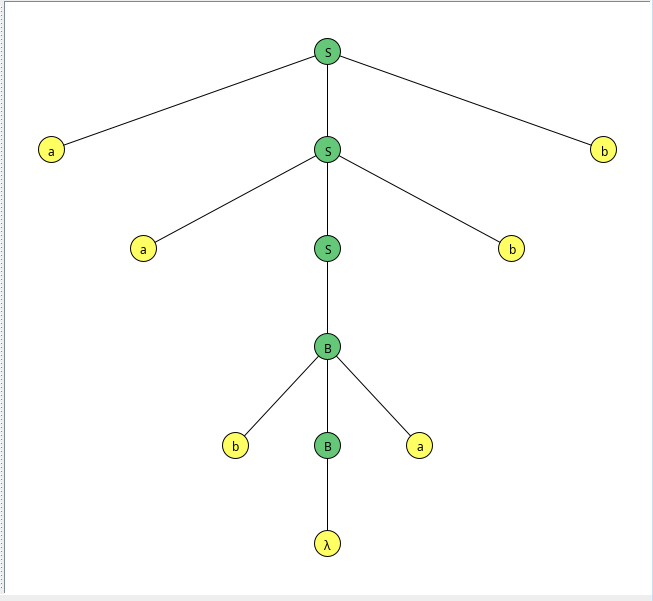
\includegraphics[width=\textwidth]{./Imagenes/grafo1.png}
                        \caption{la cadena $aababb$}
                        \label{fig:label7}
                    \end{subfigure}
                    \hfill
                    \begin{subfigure}[b]{0.45\textwidth}
                        \centering
                        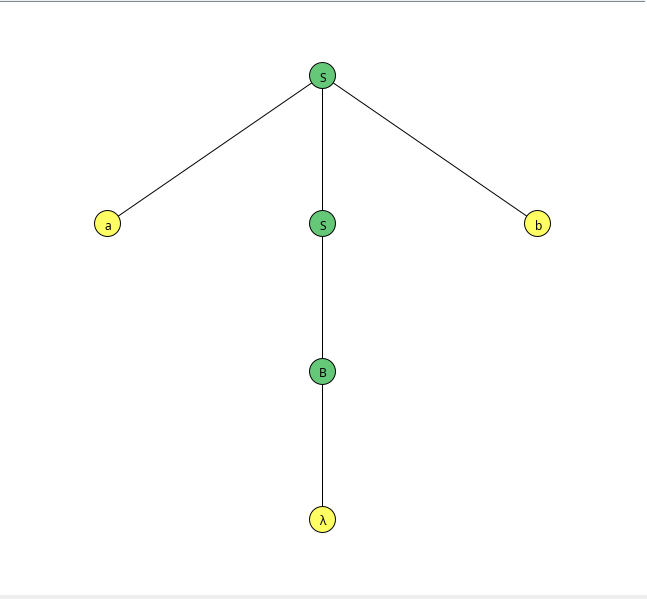
\includegraphics[width=\textwidth]{./Imagenes/grafo2.png}
                        \caption{la cadena $ab$}
                        \label{fig:label8}
                    \end{subfigure}
                    \label{fig:matrix2}
                \end{figure}

            \end{enumerate}
        \end{flushleft}
        
        
        % 
        % Apartado 3
        \newpage % paso pagina
        \subsection*{C. $L = \{a^i b^i a^j b^j \, | \, i, j \in \mathbb{N}\}$.}
        \begin{flushleft}
            \begin{enumerate}
                \item Los símbolos terminales serán $\{a,b\}$ y los simbolos no terminales serán $S$ y $B$.
                \item El símbolo inicial será $S$.
                \item El lenguaje nos pide generar cadenas de 4 caracteres de la forma $abab$ donde los dos primeros caracteres tengan 
                el mismo nuemoor de caracteres y para los dos ultimos caracteres tambien tengan la misma cantidad.Ejemplos de cadenas serían $aabbaabb$ ,$aabbab$ pero no acepta $aaba$
                \item Determino las reglas de producción:
                \begin{itemize}
                    \item $S \rightarrow AA$ (simbolo inicial).
                    \item $A \rightarrow aSb$. (genero $\{a^i b^i | i \in \mathbb{N}\}$).
                    \item $A \rightarrow \epsilon$ (genero la cadena vacía).
                \end{itemize}

                \item compruebo con JFLAP que la gramática es correcta.
                

                % Imagenes en matriz
                \begin{figure}[h] 
                    \centering
                    \begin{subfigure}[b]{0.45\textwidth}
                        \centering
                        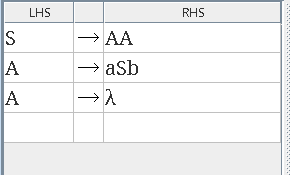
\includegraphics[width=\textwidth]{./Imagenes/produccion3.png}
                        \caption{la producción}
                        \label{fig:label10}
                    \end{subfigure}
                    \hfill
                    \begin{subfigure}[b]{0.45\textwidth}
                        \centering
                        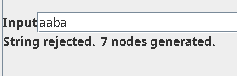
\includegraphics[width=\textwidth]{./Imagenes/grafo6.png}
                        \caption{la cadena $aaba$}
                        \label{fig:label11}
                    \end{subfigure}
                    \vspace{0.5cm} 
                    \\
                    \begin{subfigure}[b]{0.45\textwidth}
                        \centering
                        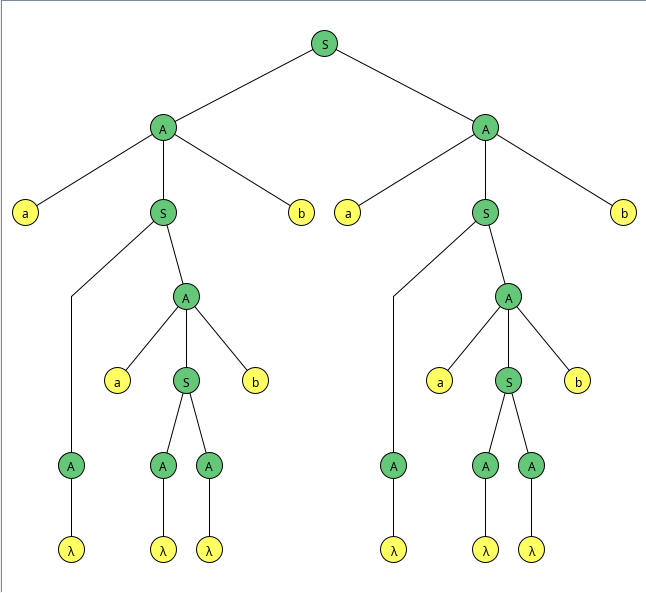
\includegraphics[width=\textwidth]{./Imagenes/grado4.png}
                        \caption{la cadena $aabbaabb$}
                        \label{fig:label12}
                    \end{subfigure}
                    \hfill
                    \begin{subfigure}[b]{0.45\textwidth}
                        \centering
                        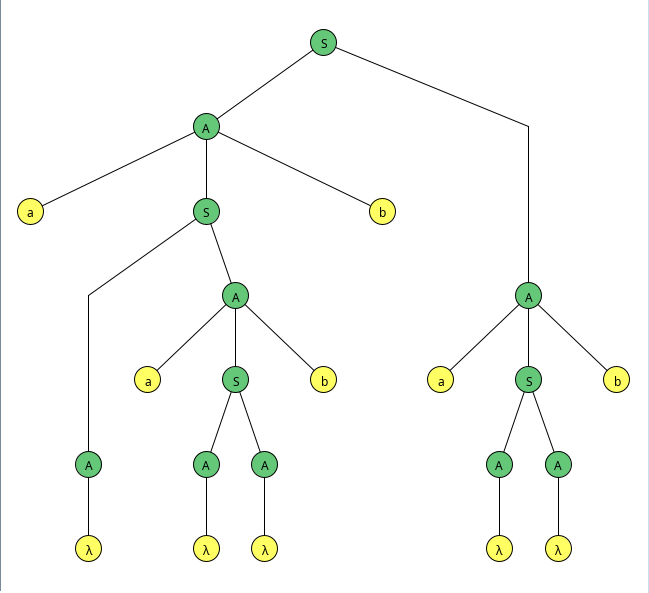
\includegraphics[width=\textwidth]{./Imagenes/grafo5.png}
                        \caption{la cadena $aabbab$}
                        \label{fig:label13}
                    \end{subfigure}
                    \label{fig:matrix3}
                \end{figure}

            \end{enumerate}
        \end{flushleft}



        % 
        % Apartado 4
        \newpage % paso pagina
        \subsection*{D. $L = \{a_i b_i \,|\, i \in \mathbb{N}\} \cup \{b_i a_i \,|\, i \in \mathbb{N\}}$.}
        \begin{flushleft}
            \begin{enumerate}
                \item Los símbolos terminales serán $\{a,b\}$ y los simbolos no terminales serán $S$ , $A$ $B$.
                \item El símbolo inicial será $S$ .
                \item Combina dos conjuntos de cadenas: el primero contiene cadenas de la forma $\{a_i b_i \,|\, i \in \mathbb{N}\}$, y el segundo contiene cadenas de la forma $\{b_i a_i \,|\, i \in \mathbb{N}\}$.Las cadenas $aabb$ $bbaa$ lo cumplen mientras $abab$ no lo cumple Lo resolvemos por partes
                \item Determino las reglas de producción:
                
                \begin{itemize}
                    \item Podemos generar $\{a_i b_i \,|\, i \in \mathbb{N}\}. $
                        \subitem $A \rightarrow aAb$ , $A \rightarrow \epsilon$. 
                    \item Por otro lado $\{b_i a_i \,|\, i \in \mathbb{N}\}$.
                        \subitem $B \rightarrow bBa$ , $B \rightarrow \epsilon$ . 
                    \item El lenguaje L se puede generar añadiendo .
                        \subitem $S \rightarrow A$ , $S \rightarrow B$ . 
                \end{itemize}

                \item compruebo con JFLAP que la gramática es correcta.
                % Imagenes en matriz
                \begin{figure}[h] 
                    \centering
                    \begin{subfigure}[b]{0.25\textwidth}
                        \centering
                        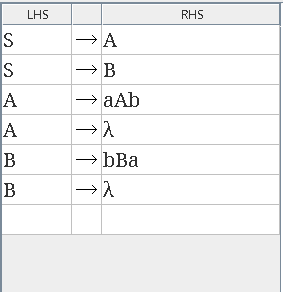
\includegraphics[width=\textwidth]{./Imagenes/produccion4.png}
                        \caption{la producción}
                        \label{fig:label14}
                    \end{subfigure}
                    \hfill
                    \begin{subfigure}[b]{0.4\textwidth}
                        \centering
                        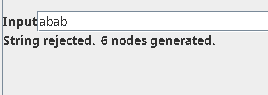
\includegraphics[width=\textwidth]{./Imagenes/grafoabab.png}
                        \caption{la cadena $abab$}
                        \label{fig:label15}
                    \end{subfigure}
                    \vspace{0.5cm} 
                    \\
                    \begin{subfigure}[b]{0.4\textwidth}
                        \centering
                        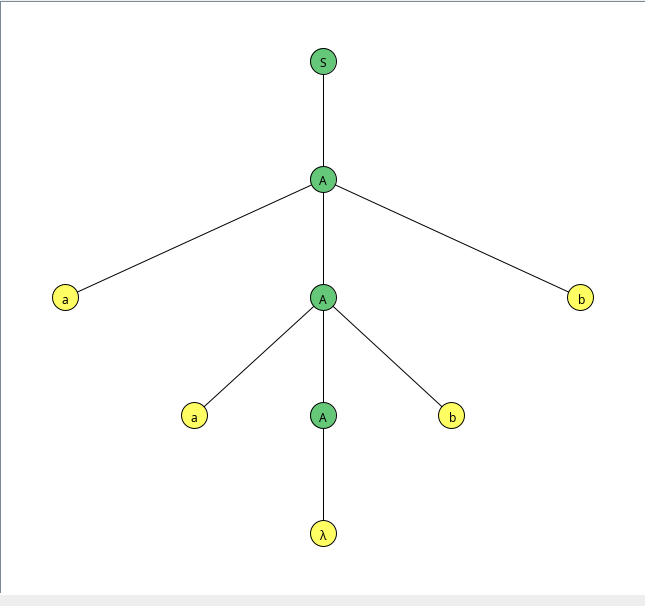
\includegraphics[width=\textwidth]{./Imagenes/grafo7.png}
                        \caption{la cadena $aabb$}
                        \label{fig:label16}
                    \end{subfigure}
                    \hfill
                    \begin{subfigure}[b]{0.4\textwidth}
                        \centering
                        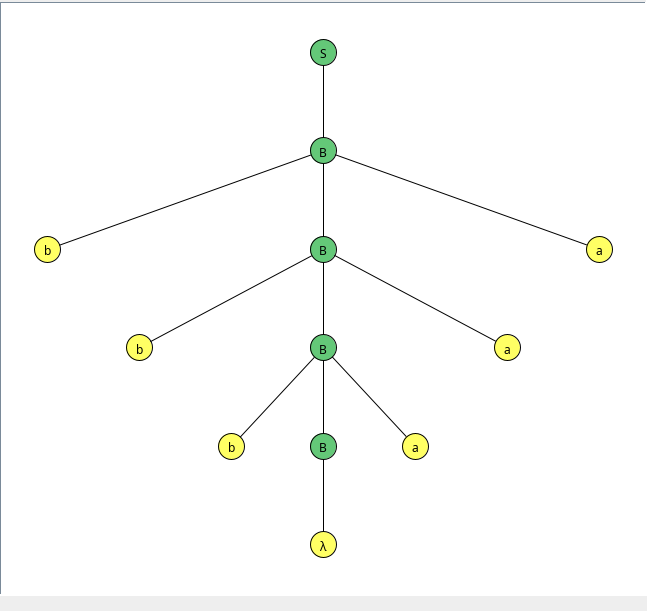
\includegraphics[width=\textwidth]{./Imagenes/grafobbbaaa.png}
                        \caption{la cadena $bbbaaa$}
                        \label{fig:label17}
                    \end{subfigure}
                    \label{fig:matrix4}
                \end{figure}



            \end{enumerate}
        \end{flushleft}
        % 
        % Apartado 5
        \newpage % paso pagina
        \subsection*{E. $L = \{uu^{-1} \mid u \in \{a, b\}^*\}$.}
        \begin{flushleft}
            \begin{enumerate}
                \item Los símbolos terminales serán $\{a,b\}$ y los simbolos no terminales serán $S$.
                \item El símbolo inicial será $S$.
                \item Analizar el lenguaje para determinar qué se pide. En este caso,se pide generar 
                cadenas que son palíndromos formados por caracteres 'a' y 'b'. Cadenas que pertenecen al lenguaje son $abba$ y $bbaabb$ pero no $bbabb$. 
                \item Determino las reglas de producción:
                \begin{itemize}
                    \item $S \rightarrow \epsilon$ (genero la cadena vacía).
                    \item $S \rightarrow aSa$.
                    \item $S \rightarrow bSb$.
                \end{itemize}

                \item compruebo con JFLAP que la gramática es correcta.
                 % Imagenes en matriz
                 \begin{figure}[h] 
                    \centering
                    \begin{subfigure}[b]{0.45\textwidth}
                        \centering
                        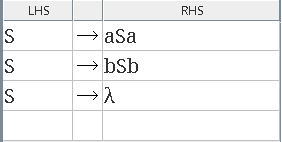
\includegraphics[width=\textwidth]{./Imagenes/produccion5.png}
                        \caption{la producción}
                        \label{fig:label18}
                    \end{subfigure}
                    \hfill
                    \begin{subfigure}[b]{0.45\textwidth}
                        \centering
                        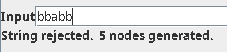
\includegraphics[width=\textwidth]{./Imagenes/grafo8.png}
                        \caption{la cadena $bbab$}
                        \label{fig:label19}
                    \end{subfigure}
                    \vspace{0.5cm} 
                    \\
                    \begin{subfigure}[b]{0.45\textwidth}
                        \centering
                        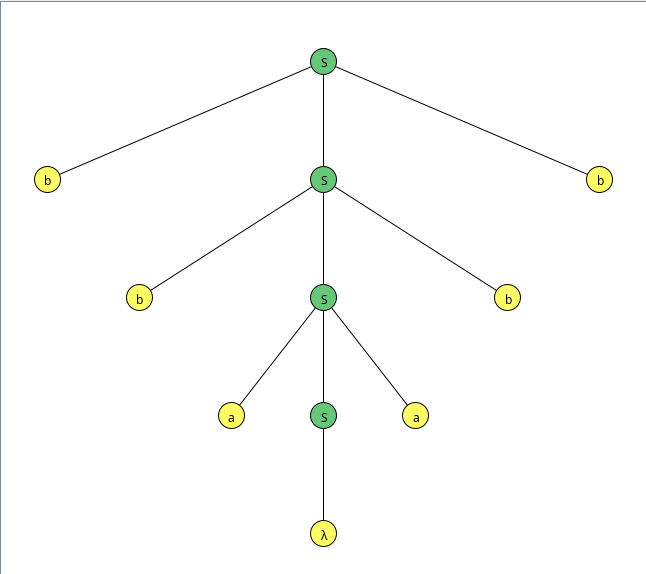
\includegraphics[width=\textwidth]{./Imagenes/grafo9.png}
                        \caption{la cadena $bbaabb$}
                        \label{fig:label20}
                    \end{subfigure}
                    \hfill
                    \begin{subfigure}[b]{0.45\textwidth}
                        \centering
                        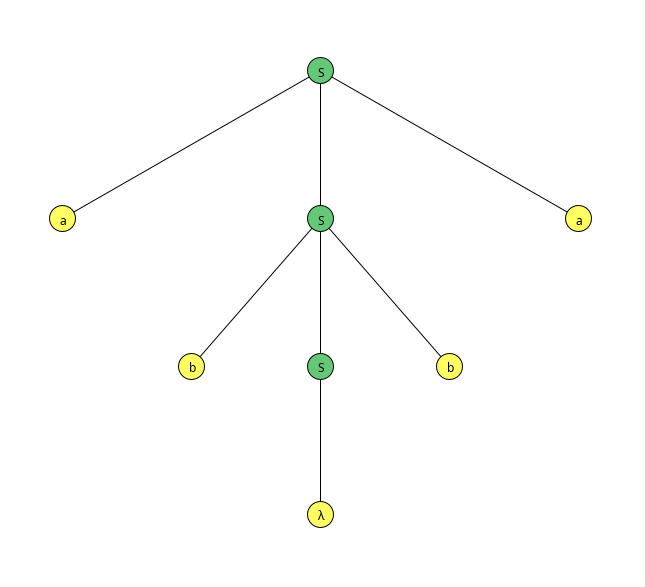
\includegraphics[width=\textwidth]{./Imagenes/grafo10.png}
                        \caption{la cadena $abba$}
                        \label{fig:label21}
                    \end{subfigure}
                    \label{fig:matrix5}
                \end{figure}

            \end{enumerate}
        \end{flushleft}

        % 
        % Apartado 6
        \newpage % paso pagina
        \subsection*{F. $L = \{a^i b^j c^{i+j} \, | \, i, j \in \mathbb{N}\}$.}
        \begin{flushleft}
            \begin{enumerate}
                \item Los símbolos terminales serán $\{a,b,c\}$ y los simbolos no terminales serán $S$.
                \item El símbolo inicial será $S$.
                \item En este caso,se pide generar cadenas donde 
                la cantidad de 'a's y 'b's es igual y la cantidad total de 'c's es la suma de las cantidades de 'a' y 'b'
                . Cadenas que cumplen la gramatica son $abbccc$ y $aaabcccc$ pero no $bacc$
                \item Determino las reglas de producción:
                \begin{itemize}
                    \item $S \rightarrow aSc$ (genero la cadena vacía).
                    \item $S \rightarrow B$.
                    \item $B \rightarrow bBc$.
                    \item $B \rightarrow \epsilon$.
                \end{itemize}
                \item compruebo con JFLAP que la gramática es correcta.
                
                % Imagenes en matriz
                \begin{figure}[h] 
                    \centering
                    \begin{subfigure}[b]{0.45\textwidth}
                        \centering
                        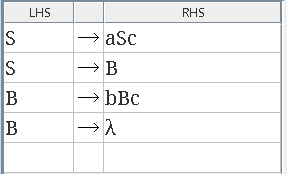
\includegraphics[width=\textwidth]{./Imagenes/produccion6.png}
                        \caption{la producción}
                        \label{fig:label22}
                    \end{subfigure}
                    \hfill
                    \begin{subfigure}[b]{0.45\textwidth}
                        \centering
                        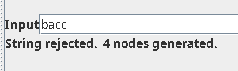
\includegraphics[width=\textwidth]{./Imagenes/grado11.png}
                        \caption{la cadena $bacc$}
                        \label{fig:label23}
                    \end{subfigure}
                    \vspace{0.5cm} 
                    \\
                    \begin{subfigure}[b]{0.45\textwidth}
                        \centering
                        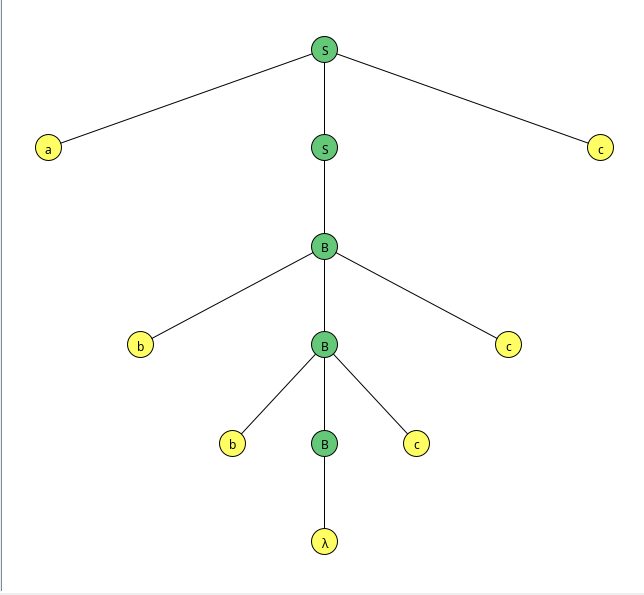
\includegraphics[width=\textwidth]{./Imagenes/grafo12.png}
                        \caption{la cadena $abbccc$}
                        \label{fig:label24}
                    \end{subfigure}
                    \hfill
                    \begin{subfigure}[b]{0.45\textwidth}
                        \centering
                        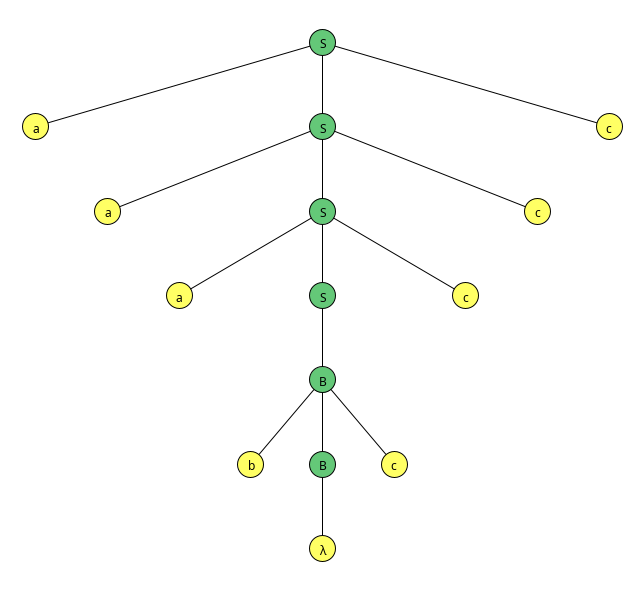
\includegraphics[width=\textwidth]{./Imagenes/grafo13.png}
                        \caption{la cadena $aaabcccc$}
                        \label{fig:label25}
                    \end{subfigure}
                    \label{fig:matrix6}
                \end{figure}


            \end{enumerate}
        \end{flushleft}


        \newpage


        %
        % PRACTICA 2
        \section*{Practica 2}
        Analizadores léxicos, problemas de mineria, trabajo Lex, 2 problema
        \subsection*{Tareas a realizar}
        \begin{enumerate}
        \item Formar un grupo de trabajo compuesto por una, dos o tres personas.
        \item Cada grupo de trabajo debe pensar un problema original de procesamiento de textos. Para la resolución de este problema debe ser apropiado el uso de Lex, o sea, se debe resolver mediante el emparejamiento de cadenas con expresiones regulares y la asociación de acciones a cada emparejamiento.
        \item Cada grupo debe resolver el problema propuesto usando Lex. Se deberá realizar una memoria donde se presente una descripción del problema y su solución, además de entregar electrónicamente los ficheros de texto con la implementación de la solución.
        \item Esta práctica deberá ser entregada antes del día 31 de Diciembre de 2020. Se entregará a través de la plataforma PRADO en un fichero .zip conteniendo todos los archivos de esta práctica. Sólo es necesario que lo entregue uno de los componentes del grupo.
        \end{enumerate}

        \vspace{\baselineskip} % paso linea


        % Pasos que voy a seguir para resolver el ejercicio
        \begin{flushleft}
            
            \subsubsection*{Pasos para resolver el ejercicio:}
                        
            \begin{enumerate}
                \item Descripcion del problema 
                \item solucion 
                \item codigo lex
            \end{enumerate}
        \end{flushleft}

        \newpage

        \subsection*{1. Descripcion del Problema}
        
        En la definición de este problema, he buscado un enfoque tanto practico como original. Desde el punto de vista de un profesor, podemos establecer, a la hora de evaluar código, una relación directa entre la cantidad/densidad de comentarios presentes en un  código fuente y la comprensión del mismo por parte del alumno, por lo que evidencia que le ha dado un mayor esfuerzo y se le podria valorar positivamente. Tambien, por otro lado es más facil evaluar el codigo sin esos comentarios, por lo que vendira bien tener una version  del código sin comentarios.Por lo tanto, el problema que se plantea es el siguiente:
    
        \subsubsection*{Densidad de comentarios y limpieza de comentarios en Codigo Fuente
        }
        Tu tarea es desarrollar un programa en Lex que calcule la densidad de comentarios en un código fuente en C. La densidad de comentarios se define como el porcentaje del código total que está ocupado por comentarios. Además, tu programa deberá ser capaz de generar una nueva versión del código eliminando todos los comentarios.


        \subsubsection*{Ejemplo}
        El alumno ha entregado su ejercicio de C correspondiente de la asignatura, voy a calcular la densidad de comentarios con la siguiente formula: 
        \[ \text{{Densidad de comentarios}} = \frac{{\text{{Longitud total de los comentarios}}}}{{\text{{Longitud total del código (sin contar los comentarios)}}}} \]
        \vspace{\baselineskip} % paso linea
        ademas voy a generar el mismo codigo pero sin texto para evaluarlo aparte.
        un ejemplo tanto de entrada como de salida será el siguiente
        
        \newpage

    
        \lstset{language=C, breaklines=true, basicstyle=\footnotesize}
        \begin{lstlisting}[frame=single]
    #include <stdio.h>
    #include <stdlib.h>
            
    // funcion de ejemplo
    void imprimirMensaje() {
        printf("! Hola, mundo!\n");
    }

    /*
        comentarios
        multilinea
    */

    int main{
        // Llamada a la funcion
        imprimirMensaje();
        return 0;
    }
    \end{lstlisting}



    \end{document}
